% CSE1_G10 | Full AI-assisted working draft for the team to rewrite.
% In Overleaf select pdfLaTeX and compile main.tex with BibTeX.
% Replace all bracketed fields. Read each cited source before submission.
\documentclass[12pt,onecolumn,draftclsnofoot]{IEEEtran}
\usepackage[a4paper,margin=1in]{geometry}
\usepackage{times,graphicx,amsmath,booktabs,cite,url}
\usepackage[ruled,linesnumbered]{algorithm2e}
\begin{document}
\title{Verifier-Guided Repair of Kubernetes Manifests Generated from Natural Language}
\author{Group CSE1\_G10\\Angelina Gupta (220456), Kavya Goswami (230467),\\
Sahil Dewani (230934), Mr. Naveen Singh sir\\
School of Engineering \& Technology, BML Munjal University}
\maketitle
\begin{abstract}
A Kubernetes manifest can pass a security scan and still describe the wrong application. This distinction matters when a language model translates an informal request into resources whose names, images and namespaces must match. We investigate whether supplying the rules in the prompt is sufficient and how many additional requests pass after bounded repair. NL2Infra keeps a structured plan, creates one manifest per planned resource and returns failed checks to the model. The application runs the checks and controls publication. Three methods handled the same 20 requests, with one reference plan shared across methods for each request. Plain generation passed the final security, policy and admission checks on zero requests. Adding the rule list raised that count to two, but both outputs differed from the plan. The full pipeline passed all four checks on 19 requests and used a median of 6,029.5 input and output tokens combined per request after planning. The remaining request produced no usable YAML. Eleven requests had three recorded repeats per method. The full pipeline passed all four checks in each repeat on this subset, which included ten easy requests. These results support targeted repair on the tested workload. Application behaviour after deployment and performance on the full hard tier remain open questions.
\end{abstract}
\begin{IEEEkeywords}
Configuration validation, infrastructure as code, Kubernetes, large language models, program repair.
\end{IEEEkeywords}
\noindent\textbf{Overleaf Project Link:} \url{https://www.overleaf.com/project/6b048d01c45f94fcc8aeaa26}

\section{Introduction}
A description of a service is usually the first part of an infrastructure request. An engineer could request a Redis cache during development, a single replica, and a port that can only be accessed within the cluster. The change typically affects more than one of the Kubernetes objects. The image and the number of replicas are controlled by the workload; the Service, by how the clients reach the replicas. A person who reads the change must understand the intended use of the change as well as the policy decisions made in the configuration. Research on natural-language generation of cloud configuration has shown that the quality of a generated manifest is plausible and that the effectiveness of the language model is dependent on the task, examples in the prompt, and the assessment metric used to evaluate the results~\cite{kgen,cloud,iac}.

A plausible file is a particular difficulty for the reviewer. If an image for the requested cache is already tested by the team, they can use that image. A model can provide another fixed tag to replace that image, provide reasonable resource restrictions, and produce a file that the cluster would accept. The reviewer will still have to notice the change of container image. A second request might be for a developer-type operator that has permission to create changes for development, but not for production. In this case the wording and role need to be double-checked prior to generation. In both of these situations, there are questions of correctness. Their remedies are at various stages and if someone makes a judgement from the model, there is not a lot of evidence to enable the reviewer to tell which one of the questions has been answered.

Existing work provides useful methods for creating files from intent, fixing configuration problems known to exist and evaluating the infrastructure generated against an external specification~\cite{kgen,sec,iac,beuter}. A narrower question remains for a team developing a review queue for Kubernetes changes. If the model already sees the applicable rules, how much work is required to turn its first draft into files that also conform to an approved plan? One question naturally follows another from a student's or engineer's experience of having to wait for that question. If an improvement is made with a further call, it will cost tokens and time. The only information that is reported is the best final file, so this doesn't show the extra effort and it also doesn't show requests that didn't have any final files.

\emph{RQ1:} How often did each of the three methods pass the safety checks, and how often did the same output also conform to the approved plan? \emph{RQ2:} How many additional requests passed all four checks when the full pipeline continued beyond its first draft, and what did the repair rounds, token counts and processing times show about the cost? We answer the first question by comparing the methods on matched requests. For the second, we compare the first and final drafts within the same run. We also use archived repeats to see how sensitive the result is to a fresh generation for the same request.


The study makes three contributions:
\begin{itemize}
\item A review workflow connects an approved resource plan to generated files and to findings from four deterministic checks. A reviewer can inspect the state that led to publication or escalation.

\item A matched comparison reports both the three check and four check results, and an empty response in the denominator. The choice of success criterion changes the conclusion because of a concrete failure.

\item A repair analysis is done between the initial and final state of the same runs and a second analysis is performed for three repeats on the whole subset of the archive. Both have the same range and expense of the recorded experiment.
\end{itemize}
The paper moves from related work and the acceptance criteria to the workflow, experimental protocol, results, limitations and next experiments.

% End of introduction.

\section{Related Work}
\subsection{Generating infrastructure from intent}
Angi et al.'s work deals with the same translation as this project, from a user's description to Kubernetes manifests \cite{kgen}. In their experiments with KGen, they vary the number of examples they provide a model. The effect varies by model: too many examples led to some specialised models being better, but may make fewer valid manifests for Llama models. This is a good indication to conduct direct measurement of the impact of additional context. Having more rules in the prompt might eliminate some common issues, but also cause some of the rules to not apply to the output. The number of findings and the fraction of requests with none is then recorded in the arm that is only concerned with following the rules.

CloudEval-YAML takes the challenge by designing a benchmark \cite{cloud}. Its authors compiled 1011 cloud-configuration problems and tested 12 models. They added variations in order to match the ways that users express their needs for assistance. IaC-Eval has another approach. Kon et al.\ also associate natural-language AWS scenarios with a specification of infrastructure intent, and report 19.36\% pass-at-one for GPT-4 on 458 scenarios \cite{iac}. Both studies motivate an explicit acceptance test. They also provide examples of the size and range that the course benchmark does not demonstrate. The percentage in the two papers should not be used to make a direct comparison between a result measured on twenty local requests and a general cloud configuration benchmark.

\subsection{Where feedback enters the process}
LLMSecConfig takes a configuration as an input that has been identified as problematic by a static analyser. To repair container misconfigurations, Ye et al. \cite{sec} use a combination of analysis, prompting and retrieval, and report success rate of 94\% for 1,000 real-world Kubernetes configurations. This is a close comparison between the repair step. The starting point for NL2Infra is one step earlier, not having a manifest to repair, and keeping the resource plan while modifying the generated text. Beuter et al. focus on the topic of explicit error report-aware Kubernetes orchestration. They notice that the feedback on the tools can correct most of the syntax and missing attributes; successive refinements can also reverse earlier improvements \cite{beuter}. This encourages using the full set of files after every repair, even if the model file was only modified to one file.

TerraFormer uses verifier feedback to construct training data and to train models for Terraform generation and mutation \cite{terra}. Its results show that infrastructure-specific training can improve correctness with respect to a base model. It answers a different engineering question from one faced by a team using a hosted model whose weights it cannot change. In the latter setting, the team controls the prompt, the conditions for accepting a result and the number of retries. Table~\ref{tab:work} compares six studies along these dimensions. Their reported outcomes refer to different tasks and different validators, so the table uses each result to identify a design choice rather than to rank the systems.

\begin{table}[htbp]\centering
\caption{Six studies that inform the choice of tasks, feedback and acceptance criteria.}
\label{tab:work}\small
\begin{tabular}{@{}p{.16\linewidth}p{.25\linewidth}p{.24\linewidth}p{.26\linewidth}@{}}
\toprule Study & Problem, method and data & Metric and finding & Scope and relevance here\\\midrule
KGen \cite{kgen} & Few-shot generation from Kubernetes intents & Manifest validity varies with model and example count & Prompt context is an experimental variable.\\
CloudEval \cite{cloud} & Unit-tested YAML generation on 1,011 problems & Tests across 12 models and request variants & Wider task coverage provides a benchmark for future transfer.\\
IaC-Eval \cite{iac} & Intent specifications for 458 AWS scenarios & GPT-4 pass@1 of 19.36\% & Terraform tasks motivate a separate intent check in Kubernetes.\\
LLMSecConfig \cite{sec} & Repair of 1,000 existing Kubernetes configurations & Reported repair success of 94\% & Starts with a faulty file. Our evaluation includes initial generation failure.\\
Beuter et al.\ \cite{beuter} & Error-aware generation for five service types & Tool feedback corrected errors. Chaining had mixed effects. & Rechecking a prior constraint matters after revision.\\
TerraFormer \cite{terra} & Verifier-guided training on Terraform generation and mutation & Reported 15.94\% improvement over its base on IaC-Eval & Training-time gains motivate testing inference-time feedback separately.\\
\bottomrule\end{tabular}
\end{table}

\subsection{What a repair experiment measures}
The source of feedback and the accounting of cost both affect the process of program generation because of the work done in general program generation. In self-Refine, generation, feedback and revision are all assigned to the same model \cite{refine}. Self-Debugging investigates the use of results and explanations to help a model correct generated programs \cite{debug}. Even when the cost of the repair is taken into account, gains on HumanEval and APPS vary widely across settings, according to Olausson et al. \cite{budget}. Based on these results, it is recommended to report the first draft along with the final answer. If that was not the case, a reader would not know if a repair process came into difficulties with drafts or if the generator had already been able to handle most of the requests before feedback comes in.

We find that, as reported in \cite{evalplus}, EvalPlus reveals incorrectness of programs when test suites are strengthened. For manifests, adding an intent check is similar, but checks a different property than executing a program. An approved plan might limit the identities and images of the resources, but leave the application-level behaviour open. Our research question is therefore specific: Given the same Kubernetes requests and fixed checks, what is the frequency of running an output that passes the checks but doesn't match the plan, and what is the frequency that a bounded series of file repairs makes both the output and plan agree. Neither the first to repair infrastructure nor the claim of operational correctness by any single checker is required for the comparison.

This will depend on the engineering decision to be made and thus the choice of baseline. An operator who has some time available for one model call can use a simple prompt or part of the input budget on rules. There is a third option, and it's for the operator with access to a cluster and a review workflow, where each planned resource has its own generation call and findings can trigger additional repair calls. A comparison of these operating options is in itself of value. To estimate the effect of a specific feedback signal, however, the starting draft must be fixed. This distinction motivates the two comparisons in our evaluation.

\section{Background and Problem Formulation}
A Kubernetes manifest is a description of the desired state. The cluster API can operate in dry-run mode, and the cluster validates and applies the admission processing to the cluster in accordance with the request, but does not persist the object \cite{api}. A successful dry run returns the answer of whether the API would accept that request, as it is currently configured. It takes more observations to start a container, to pull an image and to serve traffic and retain data after a restart. Static analysis is the other type of evidence. Checkov scans Kubernetes manifests for configuration issues~\cite{ckv}. Conftest is a test that evaluates structured configuration using policies written in Rego, which allows a team to state conditions over the submitted objects \cite{ct,rego}. Any candidate may have these checks performed on them prior to anyone being asked to merge them.

Let \(q\) represent the text of a request, \(u\) the role of the user, \(P\) the approved plan, and \(F_t\) the set of candidate files after t rounds of the repair. The inputs to the interactive system are the pair \((q,u)\). Success is a series of validated files presented for review and a record of the plan and checks. Rejection at any stage before and after the generation, and escalation after generation are also valid results. A plan includes the descriptions of resources, such as kind, name and namespace (if applicable). It can also restrict the selections (e.g., an image or a replica count). The user's intent can be inferred from the agreement with those fields. There is a recognizable limit on this proxy, as a misinformed or underspecified plan can be ratified.

For an evaluable draft, write \(S(F_t)=1\) when its files are parseable, contain resources, have scan coverage, and clear the configured Checkov, policy and server-side checks. Let \(C(F_t,P)=1\) when the plan checker also finds agreement on its tested properties. Acceptance for the primary four-check comparison is
\begin{equation}
 A_t=S(F_t)\,C(F_t,P).
 \label{eq:accept}
\end{equation}
Both are binary variables. If there is no output, it receives 0 in a request-level pass rate and a failed checker will fail to set a passing verdict. The equation in ~\eqref{eq:accept} is valid for the recorded experiment. The current implementation allows to impose the project-specific requirements if a project profile is provided. Those extra checks focus on a wider issue and are accompanied by an extra benchmark protocol.


\section{Proposed Methodology}
\subsection{Roles of the model, application and reviewer}
All actions that interact with external systems, along with application state, are owned by the application. The model sends text back via a service that logs its calls. The interactive path checks in scope, prompt injection signs, permissions and rate limits. An allowed request is sent to the planner and the planner generates structured resource descriptions. Pydantic will validate that structure prior to presenting the plan to the reviewer. Approval saves a copy of the plan. That copy stays fixed during repair so the reviewer can check whether the revised files still implement the approved decision.

Figure~\ref{fig:architecture} shows the components that exchange data around the workflow. In particular, the application can send a manifest to the Kubernetes API for a dry run while the model receives only text and structured feedback. The separate path to the Git review queue identifies the action taken after validation.
\begin{figure}[htbp]\centering
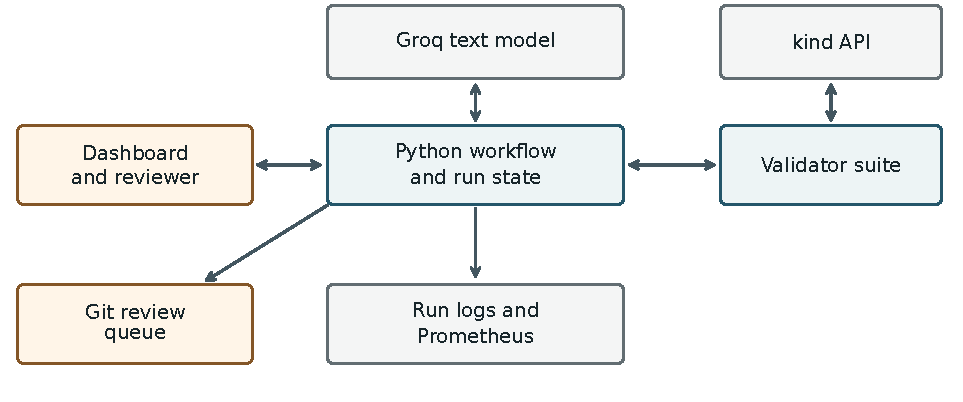
\includegraphics[width=.98\linewidth]{figures/architecture.pdf}
\caption{Component boundaries in the interactive system. The validator owns the dry-run call to kind.}
\label{fig:architecture}
\end{figure}

If a plan is approved, the generator will send out a call for each of the resources planned. The name of file that is assigned to a resource is stable across validation and repair, so the candidate that generated the finding can be associated with the finding. This option includes multi-resource requests. It also provides one special correction: If it finds a finding attached to a Deployment, it does not have to generate yet another acceptable Service. Even with the generation of resources, there are still cross-resource properties to be checked. For example, an agreement on a name for a Deployment doesn't necessarily imply that a service was generated for the deployment. The validator thus gets the full set on each round.

\subsection{Validation and bounded repair}
The four checks are for different purposes. Plan conformance identifies resources that are not included or are not planned for in the plan and differences between the fields the checker is responsible for and the resources included in the plan. Checkov looks for known configuration issues. Local Rego policies state conditions which are related to the environment or role of the project. Lastly, a server-side dry run passes candidate objects to the configured kind API. The validator stores failure data in the same common format with a tool, rule identifier, message and file association if applicable. It also documents the amount of candidate that could be scanned. This will avoid that a clean verdict will be returned in case no ordinary findings are found by the scanner, but avoid giving an empty output or a parse failure the same verdict.

There are two Checkov exclusions defined in the configuration. One is about the digest requirement. The project will be able to store a digest provided in an approved image reference, but the project won't be able to generate a valid digest for an arbitrary requested tag. The other is whether or not there is an associated NetworkPolicy. To add that resource without restriction may be in conflict with a plan that was never authorized to add that resource. The exclusions are rather narrow, and thus limit the meaning of the reported pass rate. They are documented with the benchmark, so that a team with more stringent image provenance and/or network isolation requirements can detect the difference prior to interpreting.

Figure~\ref{fig:workflow} follows one request through generation, validation and revision. Its return edge goes back to a scan of every file, which allows a correction that introduces another fault to be caught on the next round. The decision to publish occurs only after the candidate satisfies the active checks.
\begin{figure}[htbp]\centering
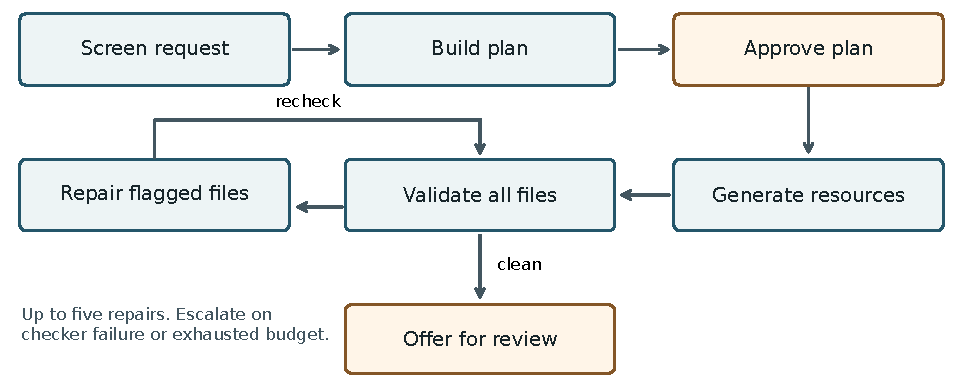
\includegraphics[width=.98\linewidth]{figures/workflow.pdf}
\caption{Interactive workflow after a request arrives. Rejection and escalation terminate the run.}
\label{fig:workflow}
\end{figure}

Algorithm~\ref{alg:repair} specifies the loop after approval. The repair prompt includes the relevant planned resource, the current file and its findings. If a rule recurs, prior file content and the earlier findings help distinguish a failed repair from a new problem. The round limit bounds the number of repair cycles. Since several files may fail in a single round, that limit alone does not bound the total number of model calls to five. The algorithm deliberately ends on checker failure. Repeatedly asking the model to repair a file cannot resolve a validator that never supplied a usable verdict.

\begin{algorithm}[htbp]
\caption{File-targeted repair after approval}\label{alg:repair}
\KwIn{Approved plan $P$, role $u$, repair budget $K=5$}
\KwOut{Validated files or an escalation reason}
Generate candidate files $F$ from the resources of $P$ for $u$\;
\If{generation produces no usable output}{\Return escalation\;}
\For{$t\gets 0$ \KwTo $K$}{
  Validate all of $F$ against $P$ and the active policies\;
  Record scan coverage, files, findings and timings\;
  \If{a checker failed to complete}{\Return escalation\;}
  \If{all active checks pass}{\Return $F$\;}
  \If{$t=K$}{\Return escalation\;}
  Group findings by file and revise affected files using $P$ and the recorded findings\;
  \If{revision fails to produce usable output}{\Return escalation\;}
}
\end{algorithm}

The workflow is extended by an optional project profile for 8 workload types. There are requirements and examples for an API, web application, static site, database, queue worker, scheduled job, one-time job and machine-learning service. If a profile is provided, the validator includes validation of required components and additional Rego rules specific to that project. If the purpose is declared, for a workload that is accepted as generic Kubernetes, further findings can be added to the workload. The implementation also features a retrieval-assisted arm which can provide policies and examples to the generator. The two features were not activated in the recorded three arm comparison. Putting them in the architecture description documents where they have evolved into the system and where the meaning of the experiment is still present.

\subsection{Review and operational evidence}
The interactive app can create a pull request to manifests repository on success. A publication error does not constitute a failed check and an operator can attempt to publish again without sacrificing previously published files as bad. This project currently has manifests that describe an Argo CD integration. The project data analysed for this paper does not include an applied Argo CD installation or a delivered project with Argo CD. Hence the evaluated outcome is concluded with validation. The benchmark also replaces a publication service which disables it from opening actual pull requests in experiments.


The implementation at commit \texttt{f33d7dd} bundles the application, Prometheus, Alertmanager and Grafana together in a Podman Compose stack. Prometheus is a tool that fetches time series from the metrics endpoint of the application \cite{prom}. The operational record documents a test alert passing through Alertmanager to an authenticated application webhook. During the status check in this review, all four services were found to be healthy and the kind control plane was running. The above observations confirm that a monitoring stack was present on the review computer. The benchmark logs predate this packaging change, so they cannot show whether moving to Podman affected latency. We subsequently added OpenTelemetry instrumentation around each pipeline stage, validation check, repair round, model call and rate-limit wait. Planning and generation have separate traces linked across the approval step, so time spent waiting for a reviewer is excluded from stage durations. In five paired mock runs, enabling an in-memory trace exporter produced the same manifests, violations, repair counts and final outcomes. Median run time was 36.4\,ms with tracing disabled and 37.3\,ms with it enabled. These measurements cover the mock pipeline. In an authenticated mock run on Podman, we retrieved both traces through Grafana and verified that the generation trace linked back to the planning trace. The stage latency panel showed nine stages. A separate run of the real validators on mock-generated manifests supplied timings for plan conformance, Checkov, Conftest and the Kubernetes server-side dry-run.

\section{Experimental Setup}
There are 30 project authored requests divided between easy, medium and hard tiers in the correctness dataset. The comparison is made between the ten easy and the ten medium requests for which each arm has a recorded first repeat. Each arm has a different number of hard-tier logs retained in the coverage: A has 6 hard-tier log requests, B has 6 hard-tier log requests, and C has 5 hard-tier log requests. That segment of the comparison is not included in the primary comparison. Table~\ref{tab:settings} indicates the settings common to the three arms and sets them apart from the later settings during the deployment review. A reader reproducing the benchmark should set the model explicitly, as there is also a model name in the code.

\begin{table}[htbp]\centering
\caption{Benchmark parameters and scope of the implementation review.}
\label{tab:settings}\small
\begin{tabular}{@{}p{.32\linewidth}p{.61\linewidth}@{}}\toprule
Setting & Recorded value or choice\\\midrule
Benchmark / review revision & \texttt{aabb0d1} / \texttt{f33d7dd} on macOS, Apple silicon\\
Hosted model / sampling & Groq \texttt{openai/gpt-oss-120b}, temperature 0.1. No fixed generation seed recorded.\\
Primary / repeat analysis & $20\times3$ arms, repeat 1 / $11\times3$ arms $\times3$ repeats, including repeat 1\\
Roles in the primary set & 7 junior developer, 12 senior developer, 1 platform administrator per arm\\
Validators & Checkov 3.3.26, embedded OPA 1.19.0, Kubernetes client and server v1.37.0. Conftest binary reports \texttt{dev}.\\
Repair limit / rule exclusions & Five rounds. \texttt{CKV\_K8S\_43} and \texttt{CKV2\_K8S\_6} skipped.\\
Execution controls & Shared reference plan per request and repeat, automatic approval in C, input guardrails bypassed, publication disabled\\
Later Podman stack & Python 3.12.13, kind v0.33.0, Podman 6.2.0. The documented VM has four CPUs and 4,096 MB.\\
\bottomrule\end{tabular}
\end{table}

Arm A asks for YAML in one call. Arm B uses the same single-call format and adds the applicable rules. Each takes the request as input and returns one document stream. Arm C uses the approved plan, generates one file per resource and can repair files after validation. All three arms are scored against the same plan for each request and repeat. B and C share the rule list, but also differ in how they generate files. To isolate the effect of continuing past the first draft with C's generator held fixed, we score C's recorded first draft as the zero-repair ablation.

Two pass rates, mean findings on the first draft, mean repair rounds and median token and time costs are reported. Individual failed checks refer to the tasks awaiting repair in the loop. Pass rates at the request level reflect if the whole candidate has passed or failed. Token counts include model input and output after shared planning. All three arms run validation. Only C includes it in the evaluator's runtime. For the scan-inclusive comparison, we add the logged validation interval to each A and B run before taking each arm's median. Both timing series exclude shared planning, human approval time and provider back-off.

For repeatability we choose request IDs that have a scored outcome for each arm for repeats 1, 2 and 3. Eleven matched IDs are generated from the main and extra-repeat archives. For each arm, we calculate the pass rate on the same eleven requests in each repeat, then report the mean and sample standard deviation of those three rates. So the same tasks are associated with each repeat. The following deterministic guardrail evaluation is performed with all 40 adversarial inputs and 30 legitimate requests. This refusal rate is not the same as the manifest acceptance rate, and is separately reported. The project evaluator reads the JSON summaries in the primary archive to be able to recreate the tables. A separate join on request identifier, arm and repeat will recreate the repeated subset from the extra archive. We confirmed that all three arms shared one approved plan for each request and repeat. The CSV is included with the results of the analysis which includes the request ID, request outcome, initial analysis results, token counts, repair rounds, and timing measures that were used in the analysis. It enables readers to modify the grouping or check a denominator, if they are not given credentials for a model. The CSV excludes prompts, generated files and the authors' local request logs.

\section{Results and Analysis}
\subsection{RQ1: Passing the configured checks and preserving intent}
Table~\ref{tab:main} reports the main comparison. The rule list reduced the average number of first-draft safety findings from 18.85 to 1.40, a substantial change even though only two of the twenty rules-only requests passed the safety gate. The distinction follows from the acceptance criterion: a draft with one remaining violation and a draft with ten both require further work before review.
\begin{table}[htbp]\centering
\caption{Primary comparison on twenty matched requests per arm, repeat one. Bold indicates the highest pass rate or lowest comparable cost.}
\label{tab:main}\small
\begin{tabular}{@{}lrrr@{}}\toprule
Outcome & A: Plain & B: Rules & C: Full pipeline\\\midrule
Scored requests & 20 & 20 & 20\\
First-draft safety pass & 0/20 & \textbf{2/20} & 0/20\\
Mean first-draft safety findings & 18.85 & \textbf{1.40} & 2.11$^{a}$\\
Final safety pass & 0/20 & 2/20 & \textbf{19/20}\\
Final plan conformance & 1/20 & 0/20 & \textbf{19/20}\\
All four checks pass & 0/20 & 0/20 & \textbf{19/20}\\
Mean repair rounds & 0 & 0 & 1.00\\
Median input tokens & \textbf{143} & 1,363.5 & 3,604.5\\
Median output tokens & \textbf{582.5} & 1,496 & 2,261\\
Median total tokens & \textbf{723} & 2,867 & 6,029.5\\
Evaluator median runtime (s)$^{b}$ & 1.7 & 4.0 & 13.0\\
Scan-inclusive median time (s) & \textbf{4.25} & 7.22 & 13.03\\\bottomrule
\end{tabular}\\[-1pt]
\begin{minipage}{.94\linewidth}\footnotesize
$^{a}$Nineteen usable C drafts. The missing draft counts as a failed request.
$^{b}$Only C includes validation in this evaluator row. Shared planning and back-off are excluded. Total-token medians are computed per run before aggregation.
\end{minipage}
\end{table}

The discrepancy between the two kinds of pass has a concrete explanation. On \texttt{easy-03}, the shared plan specified \path{memcached:1.6-alpine}. The rules-only manifest used \path{memcached:1.6.9}. It also introduced a Namespace and a ServiceAccount outside the plan. Checkov, the active Rego policies and the server dry run all accepted the result. None of those findings establishes whether an operator authorised a different image or those additional objects. An intent check supplied the missing evidence. Conversely, one plain output matched its plan but failed safety. Reporting either gate in isolation would have hidden one direction of disagreement.

Figure~\ref{fig:outcomes} places initial safety, final safety and final four-check acceptance on the same scale. B's two initial safety successes persist to its final safety column because it has no repair stage. Both disappear when the plan is included, while the nineteen successful C requests also meet the stricter endpoint.
\begin{figure}[htbp]\centering
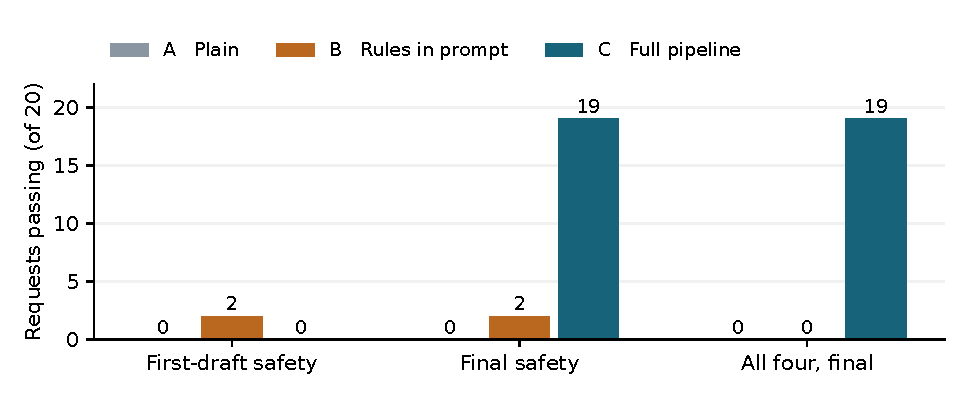
\includegraphics[width=.97\linewidth]{figures/outcomes.pdf}
\caption{Requests passing each endpoint in the first repeat. Counts above bars include explicit zeros.}
\label{fig:outcomes}
\end{figure}

\subsection{RQ2: Effect and cost of continuing past the first draft}
For the zero-repair ablation, we score arm C's first draft for each request. Before repair, zero of the 20 requests passed all four checks. After the recorded repairs, 19 of 20 passed, a gain of 95 percentage points. Eighteen requests passed after one repair round and one passed after two. The remaining request, \texttt{med-08}, was for a MongoDB StatefulSet, a Service and a Secret. Generation produced no usable YAML, so there was no draft to repair. The mean first-draft findings in Table~\ref{tab:main} use the 19 usable drafts. The pass rates include all 20 requests.

For all rounds, the Checkov rule \texttt{CKV\_K8S\_40} was mentioned in 18 different requests and \texttt{CKV\_K8S\_38} in 17. All useful first drafts showed at least one finding on the four checks. Following one repair round, there was still only one request with a finding. The number of rounds required for most of the requests is relatively small, and the few rules used are recurrent in the tasks. Other workloads may require more rounds. The difference between B and C also reflects C's use of the approved plan during generation and its use of a separate file per resource. That is the ambiguity that the within-C comparison eliminates.

There was a cost to additional calls. Median total tokens rose from 2,867 in B to 6,029.5 in C. With validation included for both arms, median processing time rose from 7.22 to 13.03 seconds. The shared planner used a median of 1,008.5 tokens per plan. The evaluator also spotted 132 attempts denied with an HTTP 429 error, and recorded wait times of around 2,568 seconds across the primary records. Those waits are the reason that a user might have a much longer wait than the timing row indicates. End-to-end request time cannot be recovered by adding up the median of each individual stage since the slowest stages may be in different stages of different requests.

\subsection{Three-repeat subset and independent input screening}
Table~\ref{tab:repeat} gives the actual numerators in each archived repeat. The rules-only arm moved between zero and three safety passes out of eleven, while every full-pipeline request in this subset cleared all four checks in every repeat. The zero observed standard deviation for C describes these three fractions and has no implication that success on an unseen task is certain.
\begin{table}[htbp]\centering
\caption{Matched subset of eleven requests. Repeat columns are counts passing safety out of eleven. The two summary columns give mean percentage $\pm$ sample SD in percentage points.}
\label{tab:repeat}\small
\begin{tabular}{@{}lrrrrr@{}}\toprule
Arm & Repeat 1 & Repeat 2 & Repeat 3 & Safety (\%) & All four (\%)\\\midrule
A & 0 & 0 & 0 & $0.0\pm0.0$ & $0.0\pm0.0$\\
B & 2 & 0 & 3 & $15.2\pm13.9$ & $0.0\pm0.0$\\
C & \textbf{11} & \textbf{11} & \textbf{11} & $\mathbf{100.0\pm0.0}$ & $\mathbf{100.0\pm0.0}$\\\bottomrule
\end{tabular}
\end{table}

The ten easy requests are matched IDs, along with \texttt{med-01}. The primary comparison contains 60 runs. The three-repeat subset contains 99 runs, of which 33 also appear in the primary comparison. Together they contain 126 distinct runs. Combining the two tables as independent evidence would double count the runs and would add extra weight to the easiest tier. In the primary comparison, C passed all four checks on ten of ten easy requests and nine of ten medium requests. The repeated subset does not include the failed medium request. This difference in coverage explains how C could pass every request in the repeated subset while achieving 95\% in the primary comparison.

The result for the input screening was different. The deterministic guardrails blocked eighteen out of forty attacks and did not block any of the thirty valid requests. Twenty-two adversarial inputs were brought to the state where the properties requested in the manifest would need to be inspected. The archive that was used for the generation comparison has a legitimate list of requests in it and can't determine how many of the twenty-two will be blocked in the end. Such a dashboard based on these measurements would be misleading because it would mix a known input decision with an unobserved outcome at the downstream end.


\section{Discussion}
A reviewer reviewing the proposed change should be aware of what makes it eligible for review. The image mismatch is more easily acted on by the memcached request than attempting to reach the general conclusion that the configuration sounds good. A policy finding, on the other hand, can refer to a specific change even if all of the resource names are accurate. Having the plan and the policy verdict separate makes each decision legible. It also provides a team with the option of asking whether the failure is an indication of the user's request, a too strict rule, an unavailable checker or a model response. Those differences help to decide who should intervene.

The benchmark prioritises tasks for which the team could identify a proposed "set of resources". The authors also implemented the system, and the evaluation was conducted only for one model and one local cluster configuration and temperature. Only one of the twenty primary requests used the platform administrator role. The same candidate's result could vary if a different admission controller or a more stringent network policy or requirement for image digests is used. C receives the shared plan during generation, whereas A and B generate from the request alone. This difference can affect the comparison of plan conformance. A and B are informative with regard to explicit rule text. The comparison of C's initial and final states is more straightforward in showing the value of repair when C's initial state is fixed.

But there are also limitations of operation and ethics. Even after being reviewed, a valid Secret object may be mis-handled and an accepted image reference may reference an application that doesn't process requests. A call to the hosted model can send part of the user's specification outside the local environment. Organisations considering such a workflow should determine what information to send in a request and who is able to view the artifacts and logs created during the process. There are fewer options for action because the model does not include direct cluster tools. Another key design consideration that cannot be overlooked is human approval, as well as the application permissions and independent management of credentials. The results corroborate a narrower engineering judgement: the four recorded checks provide evidence for the review of a proposed change under a set of policies tested.

One of the practical issues of reproducibility is what remains in the version control system. The code and prompt templates may be checked out by revision and the detailed request histories are stored locally and the hosted provider controls the serving of models. The per-run summary provided with this paper enables the ratios and medians reported to be audited separately from that service. It would be a more solid requirement if it could be reproduced a certain generated file. This would need a stable generation environment and the underlying record. This is why it's important to keep the observed failure even if a later request for the same type of failure succeeds.


\section{Conclusion and Future Work}
For RQ1, plain generation passed the three safety checks on zero of twenty matched requests, rules in the prompt passed on two, and the full workflow passed on nineteen. Both rules-only successes differed from the approved plan. All nineteen full-pipeline successes also passed plan conformance. For RQ2, stopping the full pipeline before repair gave zero four-check passes. Allowing the recorded repairs raised that count to nineteen, with a median of 6,029.5 tokens per request after planning. The remaining request produced no usable YAML. For the eleven requests with three recorded repeats, the full workflow passed all four checks in every repeat. Ten of those requests were easy.

We propose two experiments. First, run balanced repeats on the medium and hard tiers and add a single-pass baseline with the same plan and per-resource prompts as the repair arm. Second, conduct an isolated deployment evaluation to test readiness, connectivity and expected application behaviour following deployment of reviewed manifests. These experiments would isolate the benefit of additional model budget and broaden the evaluation beyond admission to the things that are important to a service owner.

\noindent\textbf{Git repository:} \url{https://github.com/angelina10504/NL2Infra}.
\par\noindent The accompanying file, \path{benchmark-summary.csv}, contains per-run outcome and cost fields for the 126 distinct recordings used in the two analyses. The raw run directories are local artifacts outside the tracked source tree.

\section*{AI-use declaration}
OpenAI Codex assisted with repository review, benchmark analysis, references, figures, LaTeX preparation. Claude code for assessing project dependencies and reaching the desired project approach.

\section*{Member contributions}
\noindent\textbf{Angelina Gupta} --- Built the dashboard, the Slack pull-request approval flow and GitHub team sign-in; ran and analysed the A/B/C benchmark; and in the final phase moved the system to Podman (kind cluster, non-root app container, hardened compose stack with Prometheus, Alertmanager and Grafana), locked dependency versions for reproducibility, fixed the alert path, and added OpenTelemetry latency tracing.\\
\textbf{Kavya Goswami} --- Built the input guardrails, the event and notification system, the first monitoring stack, retrieval over policies and run logs (arm D), the expanded benchmark datasets and evaluation charts, CI with AI-assisted PR review, the GitOps and ArgoCD configuration, and Project-Aware Generation.\\
\textbf{Sahil Dewani} --- Wrote the project report, including the literature survey of related work and the comparison of NL2Infra with industry tools and practices.

% Overleaf sharing (not printed): invite [faculty BMU email] as an editor.
\bibliographystyle{IEEEtran}
\bibliography{references}
\end{document}
